\section{Aufbau und Durchführung}
Der erste Teil des Versuchs war es fünf verschiedene Kennlinien durch Variation der Heizleistung zu bestimmen.
Dazu wurde die Schaltung aus Abbildung \ref{fig:aufbau1} verwendet.
Dabei wird eine gewählte Heizleistung mit dem regelbaren Konstantspannungsgerät eingestellt und pro gewhälter Heizleistung 20 oder mehr Werte pro Kennlinie aufgezeichnet.
Diese Messung wird für 4 verschiedene Heizleistungen wiederholt.

\begin{figure}[h]
    \centering
    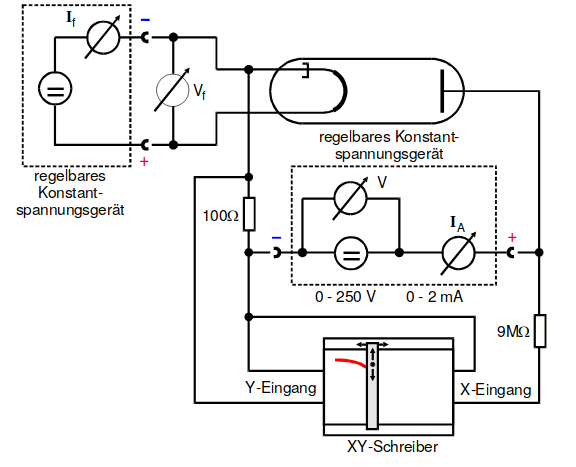
\includegraphics[height=4cm]{Durchführung/Aufbau1.png}
    \caption{Schaltung zur Messung der Kennlinie.}
    \label{fig:aufbau1}
\end{figure}

Im zweiten Teil des Experiments wurde bei maximaler Heizspannung erneut nach Abbildung \ref{fig:aufbau1} eine Kennlinie aufgezeichnet.
Hierbei wurden 40 Werte aufgenommen um damit den Bereich der Gültigkeit des Langmuir-Schottkyschen Raumladungsgesetzes zu identifizieren.
Im nächsten Versuchsteil wurde das Anlaufstromgebiet anhand Abbildung \ref{fig:aufbau2} untersucht.
Hierbei wird ein geringes Gegenfeld erzeugt und der Anodenstrom mit einem Nanoamperemeter gemessen.

\begin{figure}[h]
    \centering
    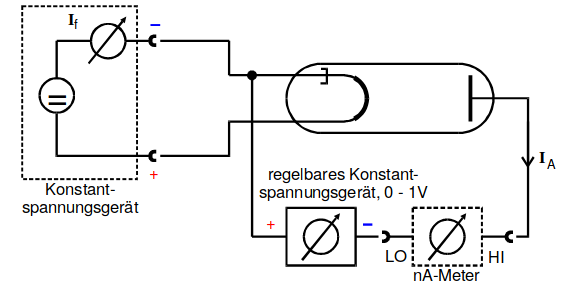
\includegraphics[height=4cm]{Durchführung/Aufbau2.png}
    \caption{Schaltung zur Untersuchung des Anlaufstromgebietes.}
    \label{fig:aufbau2}
\end{figure}